\documentclass{beamer}
\usepackage{lmodern}  % text format combination, bold+it
\usetheme[progressbar=frametitle]{metropolis}
\setbeamertemplate{frame numbering}[fraction]
\useoutertheme{metropolis}
\useinnertheme{metropolis}
\usefonttheme{metropolis}
\usecolortheme{spruce}
\setbeamercolor{background canvas}{bg=white}
\usepackage{multicol}
\usepackage{amsmath}  %math staff
\usepackage{graphicx}  %import images
\usepackage{float} %control float positions
\usepackage{amsbsy}
\title{Simulation Report 1}
\author{Jinxi Liu}
\begin{document}
	\metroset{block=fill}
	
\begin{frame}
	
	\titlepage
	
\end{frame}


\begin{frame}[t]{Introduction}\vspace{10pt}
Suppose we have $z_i \sim N(0,1)$, $i=1,2$ under the null. Their correlation is $\rho$. We perform a one-sided test with rejection region $\Gamma = \{z \geq 1.645\}.$

We then estimate $FDR(\Gamma)$ by 
\begin{equation}\label{eq1}
 \hat{FDR}(\Gamma) = \frac{\hat{\pi}_0 E[R^0(\Gamma)]}{ R(\Gamma)\vee 1}
\end{equation}

\end{frame}

\begin{frame}[t]{Empirical FDR vs Correlation}\vspace{10pt}

\begin{figure}[h]
	\centering
	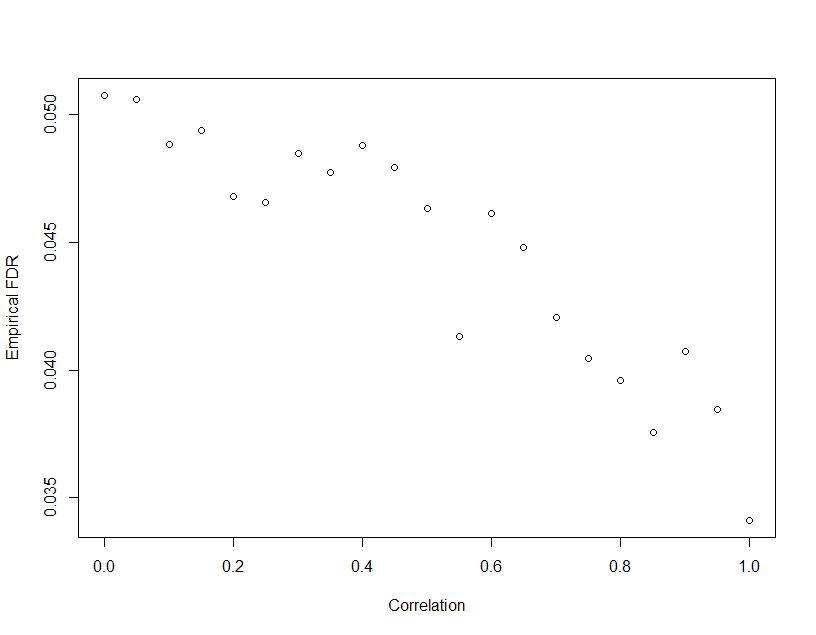
\includegraphics[scale=0.35]{fdrmeanVSrho_m=3}
	\caption{\footnotesize{Empirical FDR vs. correlation when m=3}}
	\label{fig1}
\end{figure}

\end{frame}


\begin{frame}[t]{Variance of Empirical FDR vs Correlation}\vspace{10pt}

\begin{figure}[h]
	\centering
	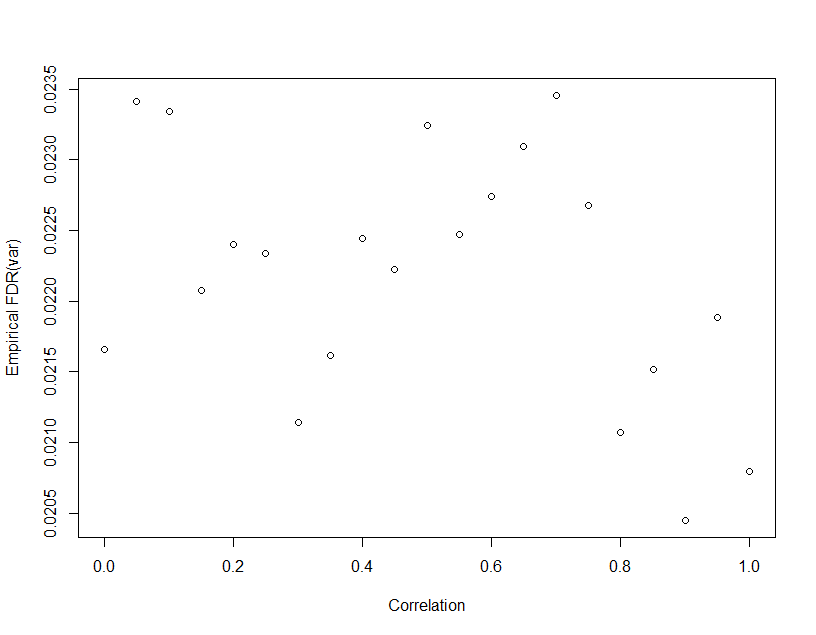
\includegraphics[scale=0.35]{fdrVarVSrho_m=3}
	\caption{\footnotesize{Variance Empirical FDR vs. correlation when m=3}}
	\label{fig2}
\end{figure}

\end{frame}

\begin{frame}[t]{Number of Rejections vs Correlation}\vspace{10pt}

\begin{figure}[h]
	\centering
	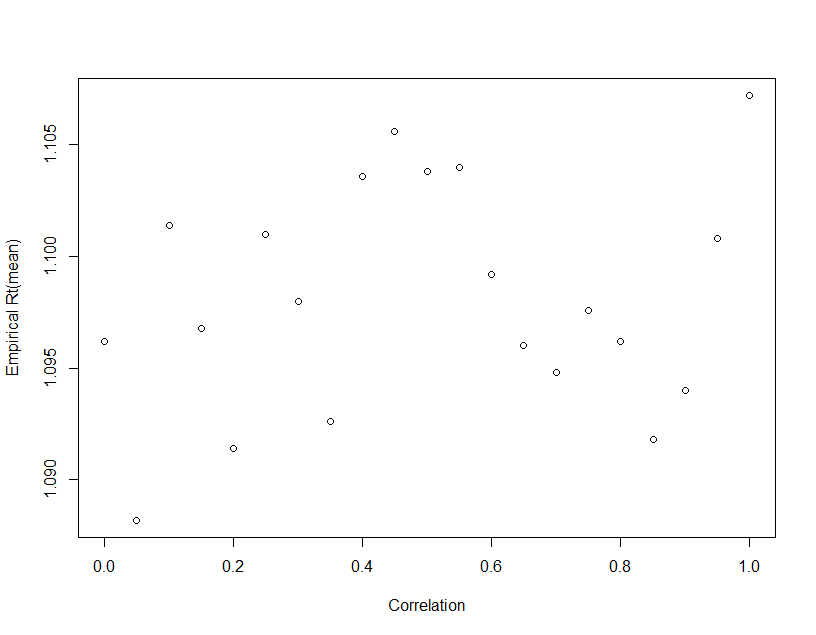
\includegraphics[scale=0.35]{rtMeanVSrho_m=3}
	\caption{\footnotesize{Number of Rejections vs. correlation when m=3}}
	\label{fig3}
\end{figure}

\end{frame}

\begin{frame}[t]{Variance of Number of Rejections vs Correlation}\vspace{10pt}

\begin{figure}[h]
	\centering
	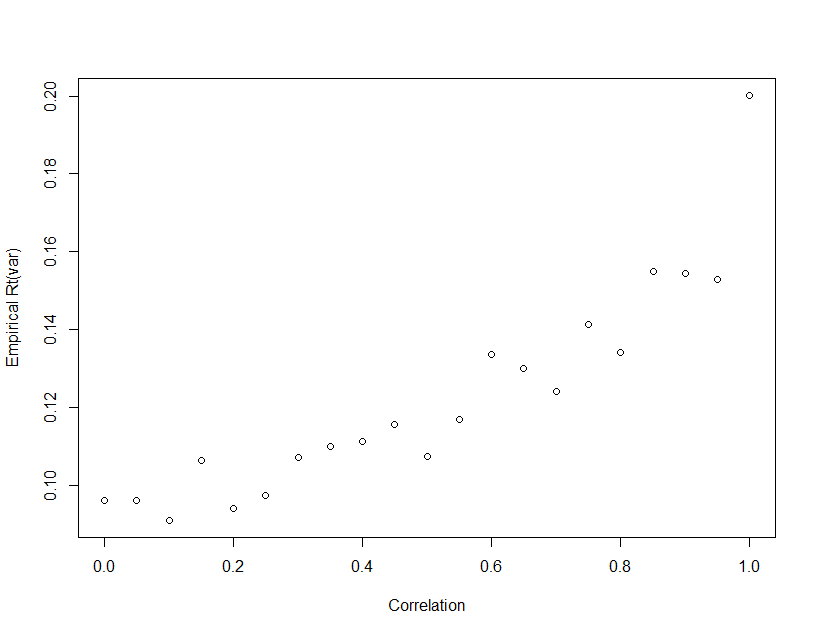
\includegraphics[scale=0.35]{rtVarVSrho_m=3}
	\caption{\footnotesize{Variance of Number of Rejections vs. correlation when m=3}}
	\label{fig4}
\end{figure}

\end{frame}


\begin{frame}[t]{Compare E(V/R) with E(v)/E(R)}\vspace{10pt}

\begin{figure}[h]
	\centering
	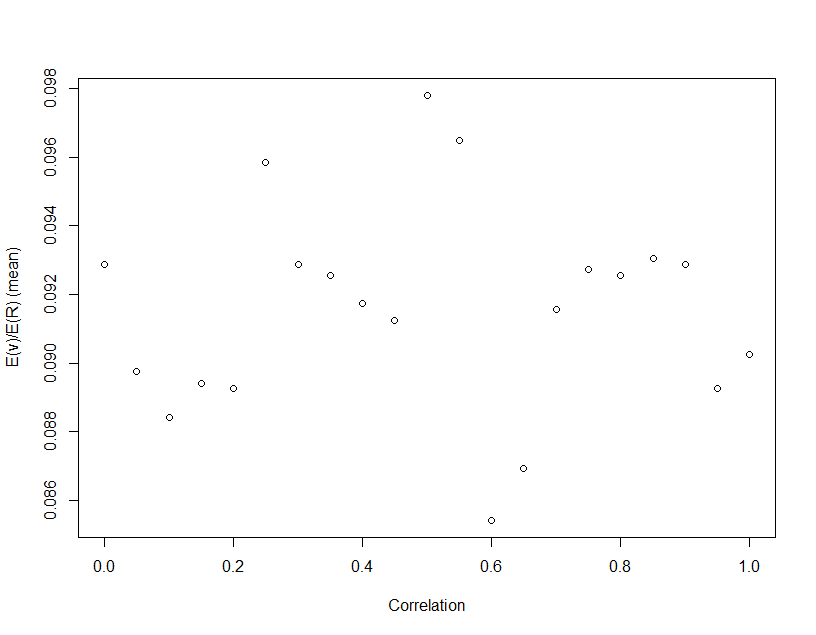
\includegraphics[scale=0.35]{EvEr_m=3_1}
	\caption{\footnotesize{E(v)/E(R) vs. correlation when $m=3$, $\mu_1=0.5$}}
	\label{fig5}
\end{figure}

\end{frame}


\begin{frame}[t]{Compare E(V/R) with E(v)/E(R)}\vspace{10pt}

\begin{figure}[h]
	\centering
	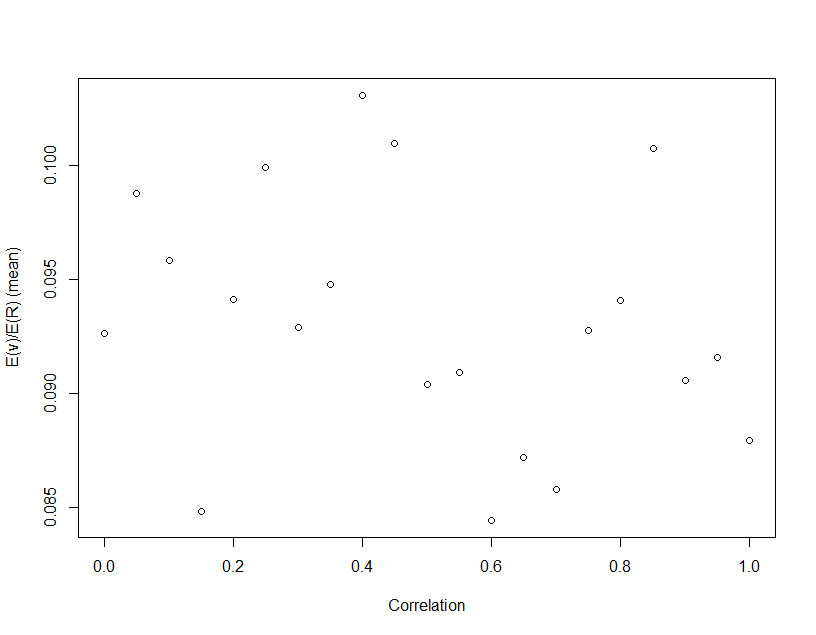
\includegraphics[scale=0.35]{EvEr_m=3_2}
	\caption{\footnotesize{E(v)/E(R) vs. correlation when $m=3$, $\mu_1=0.1$}}
	\label{fig6}
\end{figure}

\end{frame}

\begin{frame}[t]{Extend to m=100}\vspace{10pt}

\begin{figure}[h]
	\centering
	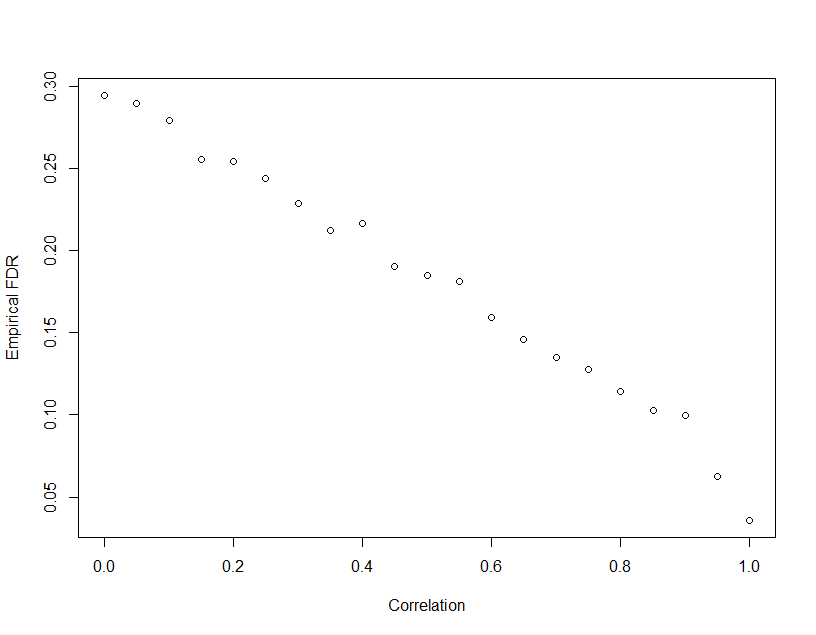
\includegraphics[scale=0.35]{fdrVSrho_m=100_1}
	\caption{\footnotesize{Empirical FDR vs. Correlation when $m=100$, $\mu_1=0.5$}}
	\label{fig7}
\end{figure}

\end{frame}


\begin{frame}[t]{Extend to m=100}\vspace{10pt}

\begin{figure}[h]
	\centering
	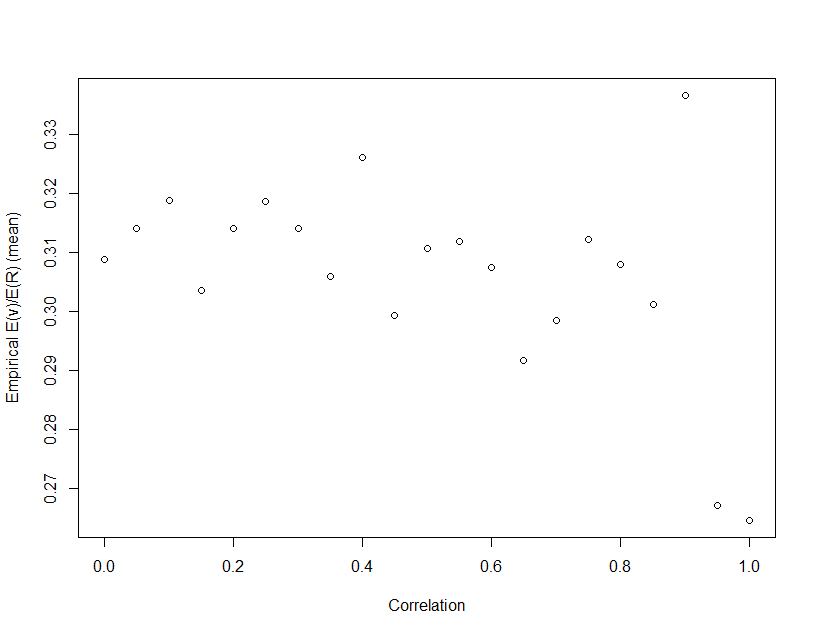
\includegraphics[scale=0.35]{EvEr_m=100_1}
	\caption{\footnotesize{E(v)/E(R) vs. Correlation when $m=100$, $\mu_1=0.5$}}
	\label{fig8}
\end{figure}

\end{frame}

\begin{frame}[t]{Extend to m=100}\vspace{10pt}

\begin{figure}[h]
	\centering
	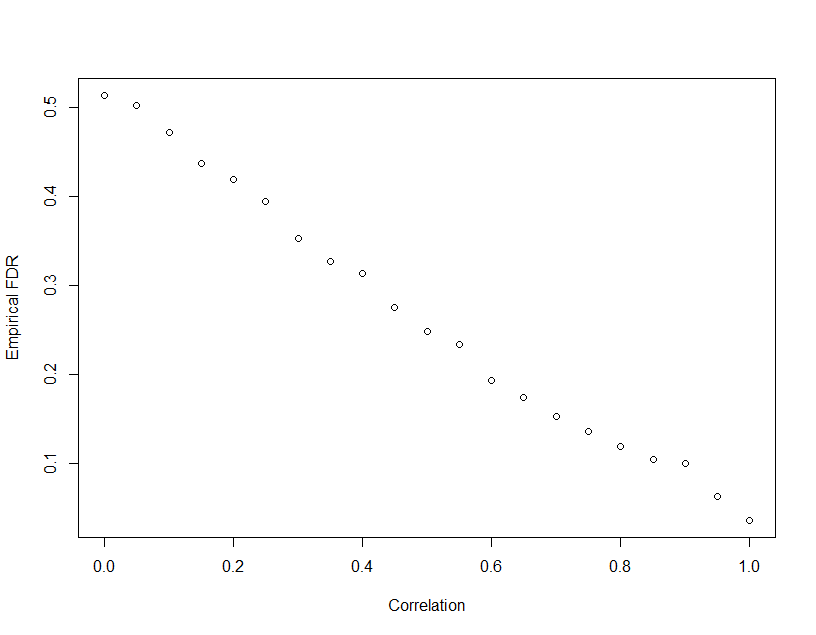
\includegraphics[scale=0.35]{fdrVSrho_m=100_2}
	\caption{\footnotesize{Empirical FDR vs. Correlation when $m=100$, $\mu_1=0.1$}}
	\label{fig7}
\end{figure}

\end{frame}

\begin{frame}[t]{Extend to m=100}\vspace{10pt}

\begin{figure}[h]
	\centering
	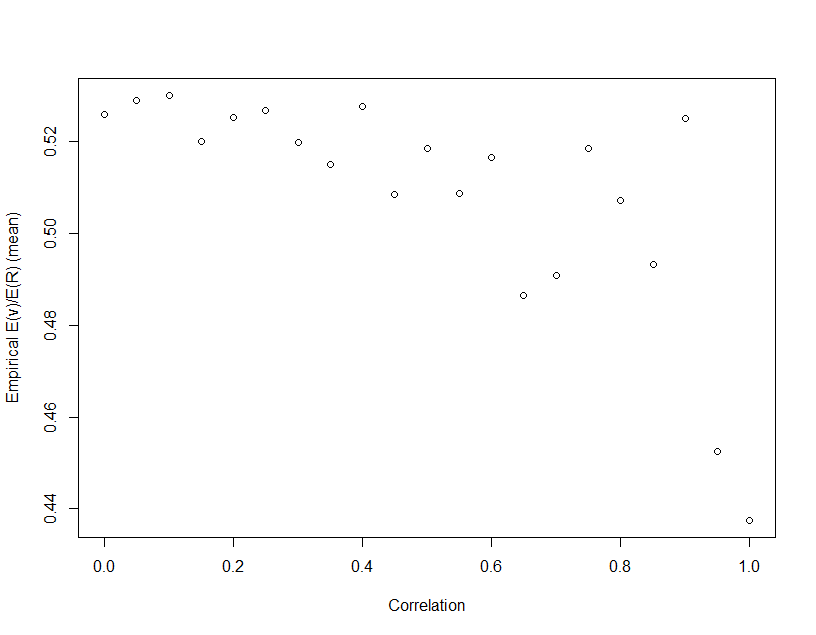
\includegraphics[scale=0.35]{EvEr_m=100_2}
	\caption{\footnotesize{E(v)/E(R) vs. Correlation when $m=100$, $\mu_1=0.1$}}
	\label{fig7}
\end{figure}

\end{frame}

\end{document}